Wir wollen noch eine weitere wichtige Anwendung f"ur die in dieser Vorlesung entwickelten Signalverarbeitungstechniken betrachten.
F"ur die Konzipierung eines RADAR-Systems macht man sich zu Nutze, dass sich ausbreitende elektromagnetische Wellen an Objekten, auf die sie w"ahren der Ausbreitung treffen, reflektiert werden.
Mit einer Antenne kann man beispielsweise ein Signal $x[\cdot]$ mit einem \gls{tx} aussenden und mit einer zweiten Antenne am \gls{rx} auf das eventuelle Echo warten.
Wird ein Objekt mit Entfernung $d$ nun von dieser Welle getroffen und reflektiert einen Teil der Energie in Richtung \gls{rx}, so enth"alt das empfangene Signal $y[\cdot]$ eine zeitlich verz"ogerte Kopie von $x[\cdot]$ und eine gewisse Menge an Rauschen, das von den Schaltkreisen an \gls{tx} und \gls{rx} eingepr"agt wird.
Es gilt also
\[
y[\cdot] = \gamma x[\cdot - \tau] + w[\cdot],
\]
wobei sich $\tau$ aus der Samplerate $F_s$, dem Abstand $d$ und der Lichtgeschwindigkeit $c$ via
\[
\tau = F_s \cdot \frac{2d}{c} 
\]
ergibt.
Die Zahl $\gamma \in \R$ repr"asentiert einerseits Verluste, die sich durch die Ausbreitung im Raum ergeben und gleichzeitig aus der \q{Reflektivit"at} des Objektes.
F"ur gew"ohnlich hat ein RADAR zwei Aufgaben. 
Einerseits soll detektiert werden, \emph{ob} ein Objekt von unserem RADAR angeleuchtet wurde und im Idealfall, wie gro"s $d$ ist.
Wir wollen uns also Signalverarbeitungstechniken ansehen, die die Bestimmung von $d$ erlauben.
%
\subsubsection{Zyklische Korrelationen}
%
Eine M"oglichkeit, um $d$ zu erhalten Basiert auf Korrelation.
Hierzu schr"anken wir zun"achst die Menge der Sendesequenzen ein, indem wir fordern, dass $x[\cdot]$ periodisch mit Periodendauer $N$ ist.
Die Korrelation $r_{x,y}$ von zwei periodischen Sequenzen $x[\cdot]$ und $y[\cdot]$ ist gegeben durch
\begin{equation}\label{eq:mseq:corr}
    r_{x,y}[\ell] = \frac{1}{N}\Sum{n = 0}{N}{
        x[n]y[n - \ell]
    }.
\end{equation}
Stellen wir uns vor, dass unser RADAR-System die Sendesequenz $x[\cdot]$ erzeugt, indem es eine endliche Sequenz $\bm x \R^{N}$ wiederholt aussendet, so ist $x[\cdot]$ periodisch mit Periodendauer $N$ und auch $y[\cdot]$ -- nach den ersten $N$ Samples.
Die Frage ist nun, was uns diese Korrelation n"utzt.
Man kann sich "uberlegen, dass
\[
\Abs{r_{x,y}[\ell]} 
    \leqslant \sqrt{
        r_{x,x}[0] \cdot r_{y,y}[0] 
    }
    = \sqrt{
        \mathcal{E}(x) \mathcal{E}(y)
    },
\]
siehe \Cref{eq:disc_sig_energy}.
Das hei"st, dass die sog.\,\emph{Kreuzkorrelation} $r_{x,y}[\cdot]$ immer durch die Werte der sog.\,\emph{Autokorrelation} $r_{x,x}[\cdot]$ wie oben angegeben beschr"ankt ist.
Im Spezialfall $y=x$ ergibt sich
\[
\Abs{r_{x,x}[\ell]} \leqslant r_{x,x}[0],
\]
was hei"st, dass die \gls{acf} $r_{x,x}[\cdot]$ ihr Maximum immer am Wert $\ell=0$ annimmt.

Betrachten wir nun wieder unser RADAR-System, so k"onnte es sich als sinnvoll erweisen, am Empf"anger das Signal $y[\cdot]$ mit dem Sendesignal zu korrelieren, also
\[
r_{y,x}[\ell] 
    = \gamma r_{x,x[\cdot-\tau]}[\ell] + r_{w,x}[\ell]
    = \gamma r_{x,x}[\ell-\tau] + r_{w,x}[\ell]
\]
zu berechnen.
Da $r_{x,x}[\cdot]$ bei $0$ ein lokales Maximum hat, so hat $r_{x,x[\cdot-\tau]}[\cdot]$ ein lokales Maximum bei $\tau$!
Wir k"onnten also einfach den maximalen Wert in $r_{y,x}[\cdot]$ suchen und dessen Stelle in $d$ umrechnen.

Die Berechnung von $r_{y,x}[\cdot]$ f"ur $N$ Werte erfordert in der Gr"o"senrdnung $N^2$ viele \glspl{flop}.
Man kann aber ziemlich einfach einsehen, dass man die Korrelation als Faltung via
\begin{equation}\label{eq:mseq:corr_conv}
    r_{x,y} = x[\cdot] \circledast y[-\cdot]
\end{equation}
ausdr"ucken kann.
Au"serdem gilt f"ur eine Sequenz $x[\cdot]$ und deren \gls{dft} $X[\cdot]$, dass
\begin{equation}\label{eq:mseq:dft_fold}
    \texttt{DFT}(x[-\cdot]) = X[\cdot]^\ast,
\end{equation}
also Umkehrung im Zeitbereich (Reflexion an $n=0$) entspricht Konjugation im Frequenzbereich.
Demzufolge k"onnen wir \Cref{par:fourier:cycl_conv} zusammen mit \eqref{eq:mseq:corr_conv} verwenden, um $r_{x,y}[\cdot]$ mit $N \log(N)$ vielen \glspl{flop} zu berechnen.
Das hei"st, dass f"ur die Signalverarbeitung effiziente Methoden bereitstehen, solange der Ansatz der Berechnung der Kreuzkorrelation des Empfangssignals mit der Sendesequenz als theoretisch fundiert herausstellt.
%
\begin{listing}[ht]
    \noindent
    \begin{minipage}{0.51\textwidth}
        \strut\vspace*{-\baselineskip}\newline
        \inputminted[firstline=6, lastline=29]{python3}{code/radar1.py}
    \end{minipage}%
    \begin{minipage}{0.48\textwidth}
        \strut\vspace*{-\baselineskip}\newline
        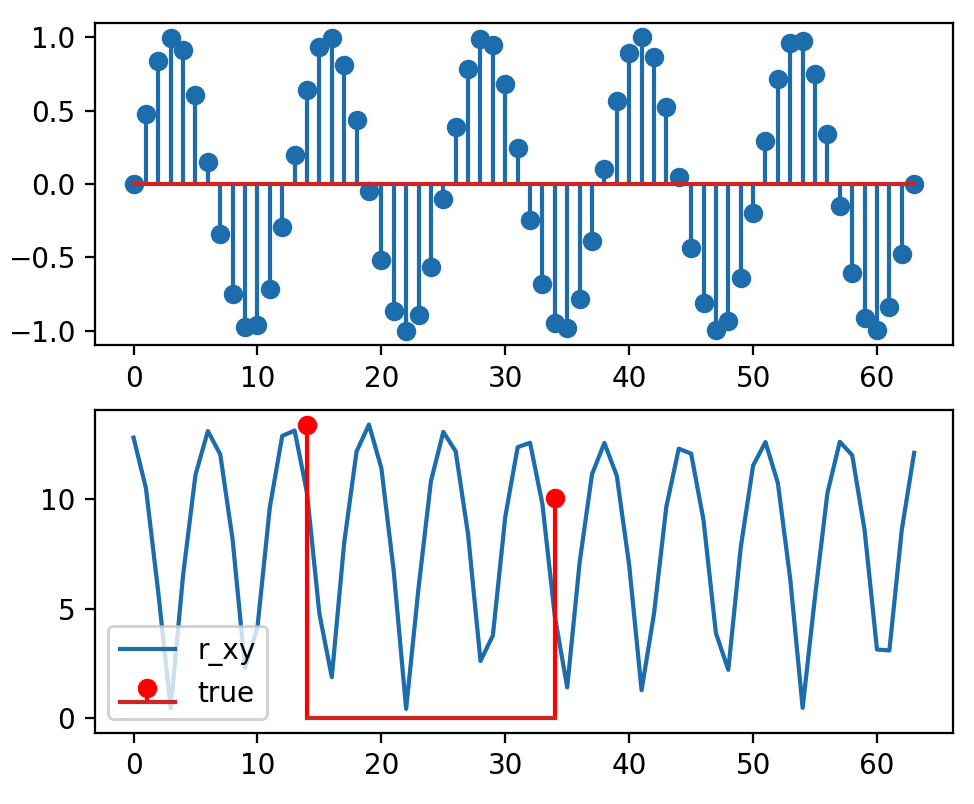
\includegraphics[width=\textwidth]{code/radar_1_1.png}

        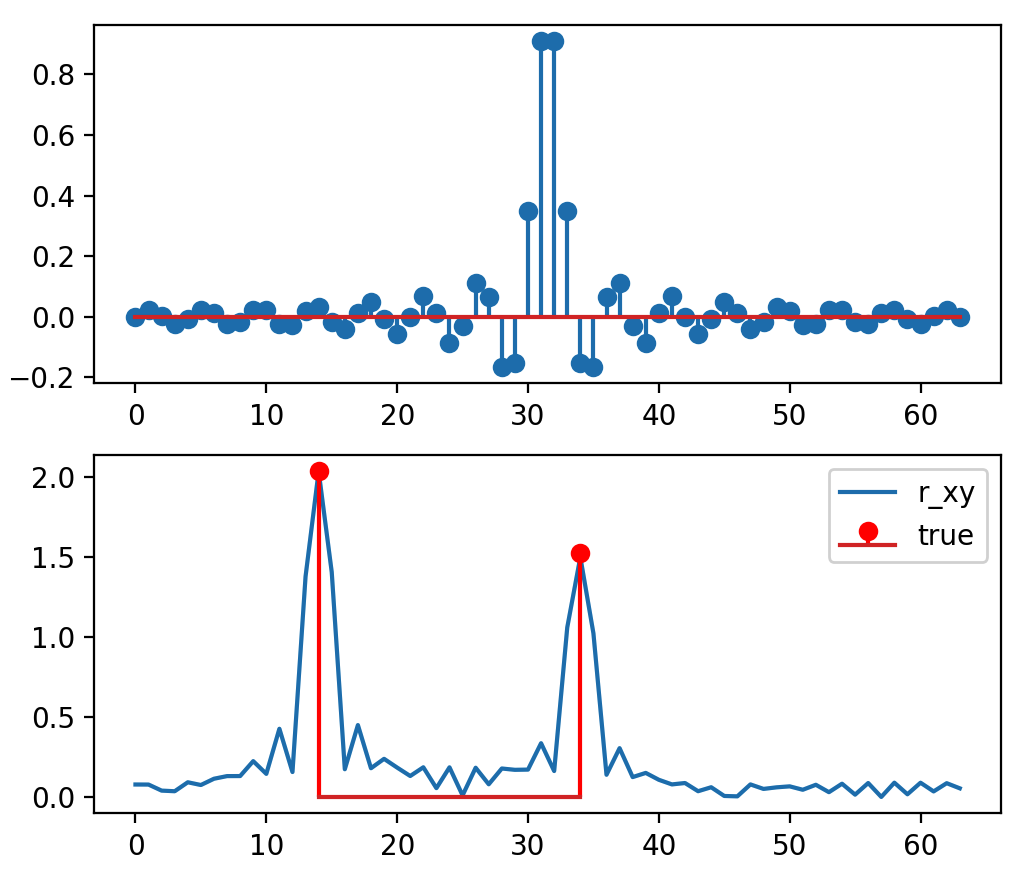
\includegraphics[width=\textwidth]{code/radar_1_2.png}

        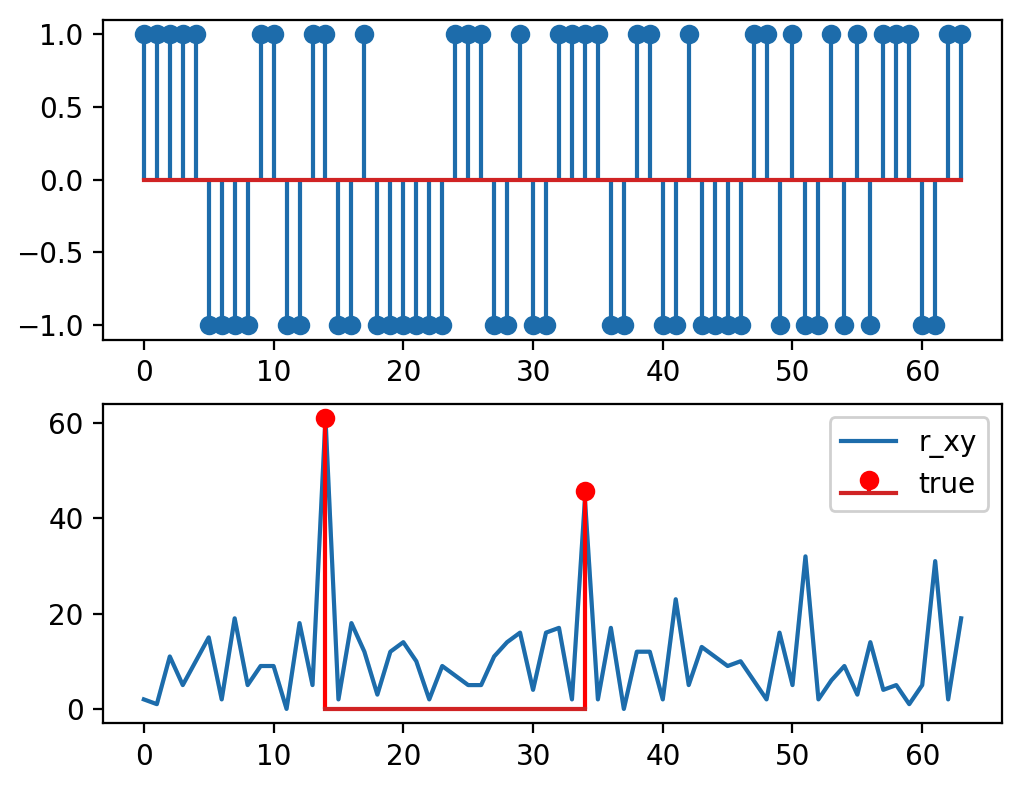
\includegraphics[width=\textwidth]{code/radar_1_3.png}
    \end{minipage}
    \codecaption{dsv/code/radar_1.py}{Vergleich verschiedener Sendesignale $x[\cdot]$ bez"uglich der resultierenden Korrelation $r_{x,y}[\cdot]$}\label{py:radar1}
\end{listing}

In \Cref{py:radar1} sind einige verschiedene Sendesignale miteinander verglichen, indem zwei Reflexionen mit verschiedenen Abst"anden simuliert werden und aus dem resultierenden Empfangssignal $y[\cdot]$ wiederum $r_{x,y}[\cdot]$ bestimmt wird.
Wie man sieht, hat das Sendesignal einen signifikanten Einfluss auf die \q{Form} der \gls{acf}, welche wiederum einen Einfluss auf die visuelle Qualit"at der Funktion $r_{x,y}[\cdot]$ hat, wenn man an die Anwendung im RADAR denkt.
Nutzt man nur einen einfachen Sinus als Sendesignal (\Cref{py:radar1}, oben), so kann man gar keine Information "uber den Abstand von eventuellen Reflexionen finden. 
Der Grund ist, dass sich Zeitversatz nur mit Signalen sch"atzen l"asst, die eine gewisse Bandbreite abdecken, also mehrere Frequenzen gleichzeitig belegen.

Mit einer $\Sinc$-Funktion (\Cref{py:radar1} mitte) belegen wir bekannterma"sen im Frequenzbereich einen kontinuierlichen Bereich, was dazu f"uhrt, dass wir in der Tat sehr ausgepr"agte lokale Maximum bei den wahren $\tau$ erhalten.
Je schmaler die Hauptkeule der $\Sinc$-Funktion im Zeitbereich, desto breiter ist der abgedeckte Frequenzbereich, was leicht durch Modifikation von \Cref{py:radar1} "uberpr"uft werden kann.
Dies ist von Vorteil, wenn man mehrere Reflexionen, die in etwa gleichen Abst"anden auftreten doch noch von einander unterscheiden m"ochte.
Es ist jedoch zu bemerken, dass ein im Zeitbereich \q{schmaler} $\Sinc$ an die Hardware, die ihn erzeugt einige unangenehme Herausforderungen stellt, weshalb solch ein Sendesignal in der Praxis einige Nachteile aufweist.

Schlussendlich sehen wir (\Cref{py:radar1}, unten), dass zuf"allige Sendesignale auch gute Eigenschaften bez"uglich $r_{x,y}[\cdot]$ liefern.
Gleichzeitig haben diese den Vorteil, dass keine gro"sen Spr"unge in der Amplitude notwendig sind, da sich das Signal bei maximaler Amplitude nicht sehr weit von seinem Mittelwert entfernt\linkfootnote{https://en.wikipedia.org/wiki/Crest_factor}.
Deren Nachteil ist jedoch, dass man kein System auf g"anzlich zuf"alligem Verhalten fu"sen lassen sollte.

Speziell f"ur unsere Anwendung im RADAR streben wir also an, dass die \gls{acf} $r_{x,y}[\cdot]$ ein ausgeptr"agtes lokales Maximum hat, also einerseits sehr schnell abf"allt, und andererseits auch wenig bis keine Nebenmaxima erzeugt, weil sich dies beispielsweise in \Cref{py:stft_harm} als Problem herausgestellt hatte.
Im Idealfall finden wir eine Sendesequenz, die sich einerseits gut f"ur RADAR eignet und gleichzeitig sich beispielsweise effizient in Hardware erzeugen l"asst.

\FloatBarrier
\subsubsection{Erzeugung der Sendesequenz}
%
\begin{figure}
    \begin{center}
        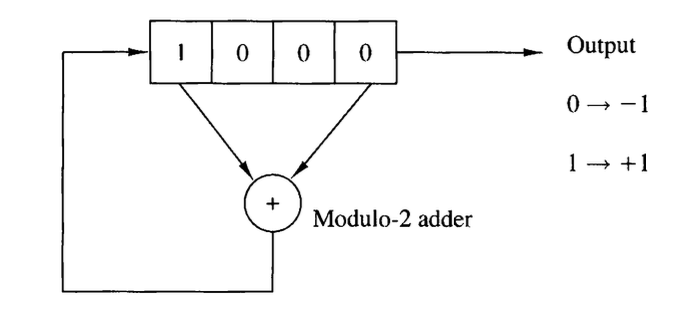
\includegraphics[width=0.6\textwidth]{img/lfsr_1.png}
    \end{center}
    \caption{Lineaeres Feedback Shift Register, Quelle \cite{proakis2013}}\label{fig:mseq:lfsr}
\end{figure}
%
Wir wollen im Folgenden eine m"ogliche Art der Sequenzerzeugung genauer untersuchen, da sie beide obigen Anforderungen erf"ullt.
Hierzu betrachten wir sogenannte \glspl{lfsr}, wie in \Cref{fig:mseq:lfsr} dargestellt.
Diese bestehen aus $L$ Registern/Taps, welche jeweil ein Bit beinhalten.
Die Idee ist nun dieses \gls{lfsr} als diskretes System zu betrachten, dessen Werte in der Menge $\Z_2^L = \{0,1\}^L$ liegen k"onnen und diese Menge $\Z_2$ mit der bin"aren Addition und Multiplikation ausgestattet wurde.
In jedem Takt werden die Werte von Links nach Rechts verschoben, wobei der Zustand des letzten Registers als Ausgabe fungiert.
Weiterhin werden einige der Zust"ande durch bin"are Addition miteinander verkn"upft und an den Eingang, also das erste Register, als Feedback zur"uckgef"uhrt.
Es ist demnach auch leicht zu sehen, dass solch ein System sehr leicht und effizient in diskreter Hardware implementiert werden kann.

Zum Zeitpunkt $n$ ist damit die Ausgabe
\[
y[n] 
    = x[n] 
      + a_1 x[n-1] 
      + \ldots 
      + a_{L-1} x[n - (L-1)] 
      + x[n-L],
\]
wobei die Koeffizienten $a_1, \ldots, a_{L-1} \in \Z_2$, also definieren, welche Werte der Register f"ur die Berechnung des Feedbacks genutzt werden.
Man kann das System zum Zeitpunkt $n$ durch die Werte $x[n], \ldots, x[n-L]$ also eine Bin"arzahl mit $L$ Stellen/Bits beschreiben. 
Kennt man all diese Zust"ande, ist es auch m"oglich den N"achsten zu berechnen, indem auf die Zahl ein Bitshift und eine \q{maskierte} Addition "uber die Bits des aktuellen Zustands angewandt wird.

Man sieht nun, dass sich mit $L$ bin"aren Registern $2^L$ Zust"ande abbilden lassen, und dass das System maximal $2^L-1$ von diesen durchlaufen kann, wenn man nicht im Zustand $0\ldots 0$ beginnt.
Die Werte $y[n]$ m"ussen demnach periodisch sein, denn sobald sich ein einzelner der $2^L-1$ m"oglichen Zust"ande ein zweites Mal einstellt, folgen ihm wieder diesselben wie beim ersten Auftreten.
Demnach ist auch die maximale Periode mit $2^L-1$ beschr"ankt.
Die Frage ist nun, ob es Koeffizienten-Konfigurationen gibt, f"ur welche die maximale Periodenl"ange erreicht wird.

Hierzu betrachten wir die $z$-Transformation des Systems, dann finden wir
\[
H(z) = 1 + a_1 z^{1} + a_2 z^2 + \ldots a_{L-1} z^{L-1} + z^L,
\]
woran wir wiederum sehen, dass das System nur durch die Wahl der Koeffizienten $a_1, \ldots, a_{L-1} \in \Z_2$ bestimmt wird.
Man kann zeigen, dass falls die Transferfunktion $H$ ein sogenanntes irreduzibles Polynom
\footnote{
    Siehe, \refurl{https://de.wikipedia.org/wiki/Irreduzibles_Polynom}. 
    Irreduzible Polynome treten im Zusammenhang mit endlichen K"orpern auf, beispielsweise $\Z_2$, wo eine andere Art Polynomdivision angewandt werden kann/muss. 
    Irreduzible Polynome nehmen im Grunde hier die Rolle von Primzahlen ein, da sich jedes Polynom in ein Produkt aus irreduziblen Polynomen zerlegen l"asst.
} ist, so hat die von diesem \gls{lfsr} erzeugte Sequenz maximale L"ange, also $2^L-1$.
Das hei"st, dass die algebraischen Eigenschaften der $z$-Transformierten der Transferfunktion $H$ wieder Aufschluss dar"uber geben, welche Eigenschaften das \gls{lfsr} als System betrachtet besitzt.
In \Cref{py:mlbs} wird ausgehend von einem Startwert des Registers (\texttt{0x1}) und einer sogenannten Tapkonfiguration (\texttt{0xD}) eine \gls{mlbs} durch einmaliges Simulieren des \gls{lfsr} erzeugt.
Die entstehende Folge hat "ahnliche Eigenschaften, wie eine \q{wirklich} zuf"allige Zahlenfolge, doch entsteht aus einem vollst"andig deterministischem Prozess.
Man nennt solche Sequenzen \q{pseudo zuf"allig}.
%
\begin{listing}[ht]
    \noindent
    \begin{minipage}{0.51\textwidth}
        \strut\vspace*{-\baselineskip}\newline
        \inputminted[firstline=5, lastline=32]{python3}{code/mlbs.py}
    \end{minipage}%
    \begin{minipage}{0.48\textwidth}
        \strut\vspace*{-\baselineskip}\newline
        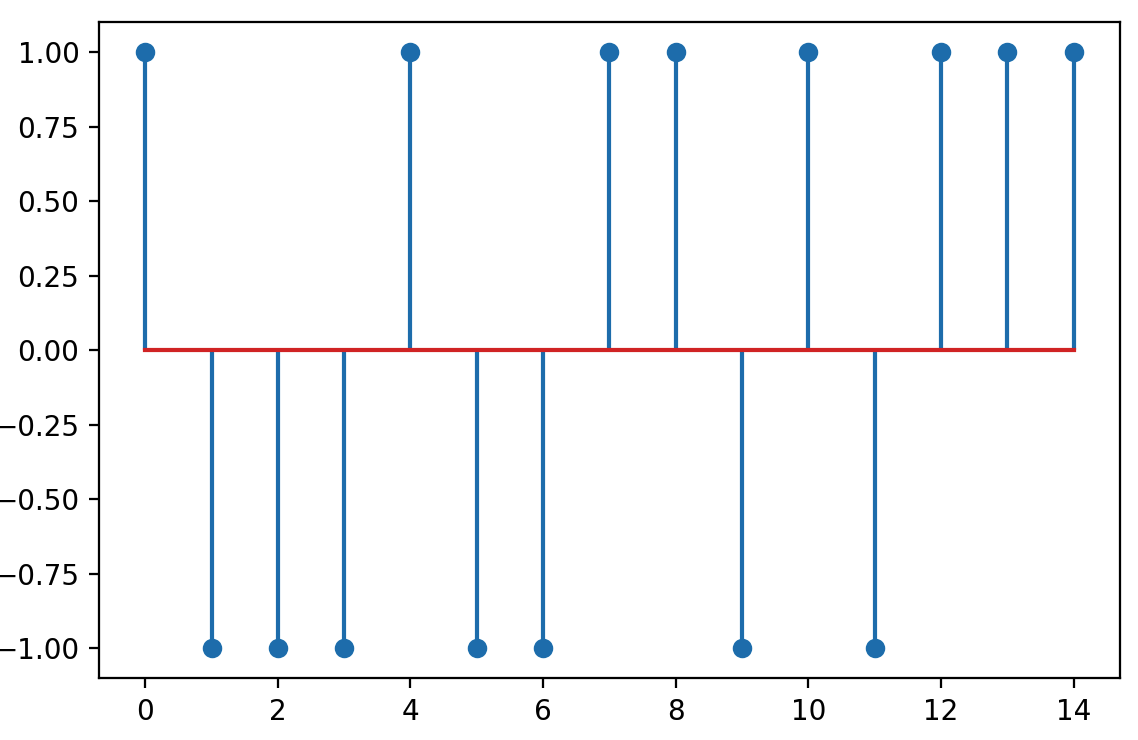
\includegraphics[width=\textwidth]{code/mlbs.png}
    \end{minipage}
    \codecaption{dsv/code/mlbs.py}{Simulation eines \acrshort*{lfsr} mittels bin"aren Operationen}\label{py:mlbs}
\end{listing}
%
\FloatBarrier
%
\subsubsection{\texorpdfstring{\acrshort*{mlbs}}{MLBS} als Sendesequenz}
Zum Abschluss wollen wir nun noch untersuchen, wie gut sich die so gewonnenen Sequenzen f"ur RADAR verwenden lassen.
Hierzu betrachten wir die Ausgabe von \Cref{py:radar2}, wo wir das Wissen aus \Cref{py:radar1} und \Cref{py:mlbs} kombiniert haben, um einerseits \q{effizient} eine
Sendesequenz zu erzeugen und andererseits, um die RADAR-Signalverarbeitung effizient zu gestalten.
%
\begin{listing}[ht]
    \noindent
    \begin{minipage}{0.51\textwidth}
        \strut\vspace*{-\baselineskip}\newline
        \inputminted[firstline=3, lastline=21]{python3}{code/radar2.py}
    \end{minipage}%
    \begin{minipage}{0.48\textwidth}
        \strut\vspace*{-\baselineskip}\newline
        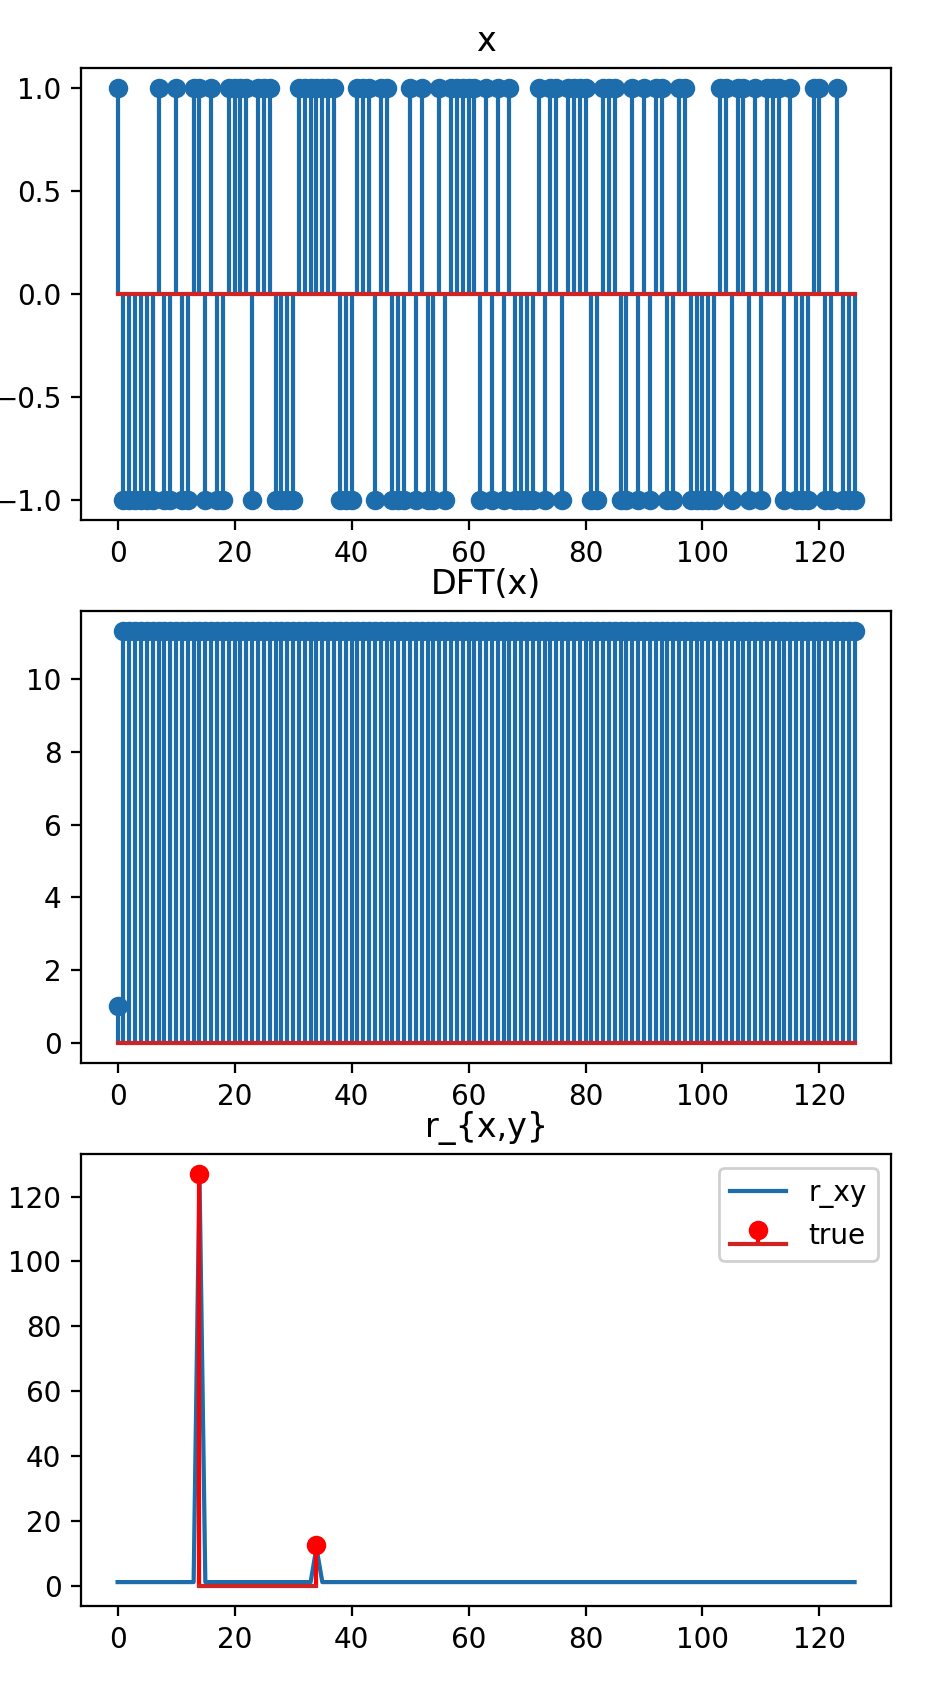
\includegraphics[width=\textwidth]{code/radar2.png}
    \end{minipage}
    \codecaption{dsv/code/radar2.py}{Simulation eines RADAR-Systems basierend auf \acrshort*{mlbs}, die von \acrshort*{lfsr} erzeugt wurden. Oben verrauschtes Empfangssignal $y[\cdot]$, mitte \acrshort*{dft} $Y[\cdot]$, unten $r_{x,y}$}\label{py:radar2}
\end{listing}

Wir wir sehen, erzeugt das \gls{lfsr} eine Sequenz, welche sehr gut zu unseren Anforderungen passt. 
Einerseits ist die Aussteuerund des Signals sehr begrenzt und andererseits hat die \gls{acf} ideale Eigenschaften, um Abst"ande von Reflexionen zu bestimmen.
Man kann sogar beweisen, dass f"ur eine Sequenz maximaler L"ange $x[\cdot]$ gilt, dass
\begin{equation}
    r_{x,x}[\ell] = \begin{cases}
        1 \Text{f"ur} \ell = 0, \\
        -\frac{1}{2^L -1} \Text{sonst.}
    \end{cases}
\end{equation}
Damit ist das lokale Maximum immer um den Faktor $N = 2^L-1$ h"oher als die Werte im Rest der Korrelationsfunktion $r_{x,x}$. 
Die bedeutet einerseits, dass dieses Verfahren auch mit eventuellem Messrauschen sehr gut umgehen kann.
Andererseits kann man auch durch den Einsatz von sehr langen Sequenzen, also mehr Registern im \gls{lfsr}, mit sehr wenig Sendeleistung durch die Transformation von $y[\cdot]$ nach $r_{x,y}[\cdot]$ immernoch Reflexionen detektieren.
